\chapter{\IfLanguageName{dutch}{Stand van zaken}{State of the art}}
\label{ch:stand-van-zaken}

% Tip: Begin elk hoofdstuk met een paragraaf inleiding die beschrijft hoe dit hoofdstuk past binnen het geheel van de bachelorproef. Geef in het bijzonder aan wat de link is met het vorige en volgende hoofdstuk.

Zoals uit vorig hoofdstuk kan worden afgeleid zal deze scriptie onderzoek doen naar de implementatie en effecten van bepaalde UX en UI-elementen. Maar alvorens van start te gaan hiermee zal eerst gekeken worden naar wat de algemene rol is van UX en UI in software-ontwikkeling.

\section{User experience in software}
\label{sec:user-experience-in-software}

In het traditioneel proces van het ontwikkelen van software staat de functionaliteit centraal. Ontwikkelaars bekijken alle vereisten en starten met de belangrijkste. Functionaliteit krijgt hier doorgaans de voorkeur. \textcite{Harutyunyan2019} stelden vast dat dit de laatste jaren echter aan het wijzigen is. De traditionele softwareontwikkeling is plaats aan het maken voor softwareontwikkeling met user experience in het achterhoofd. Dit fenomeen noemt men User Experience Design of kortweg UXD. Omdat de term UXD in de literatuur nog sterk evolueert heeft dit nog geen algemeen aanvaarde definitie. Men kan stellen dat user experience design een proces is waarbij men gebruiksgedrag zal manipuleren aan de hand van de bruikbaarheid en wenselijkheid in de interactie met een product. 

Men doet al lang onderzoek naar user experience in software. Zo toonden \textcite{Carroll1984} het belang van training in complexe systemen al aan anno 1984. Deze training van gebruikers behandelen we later in dit hoofdstuk.

\begin{figure}[h]
    \centering
    \def\svgwidth{.8\columnwidth}
    \input{./img/user-experience-waarom-wat-hoe.pdf_tex}
    \caption{Het waarom, wat en hoe van user experience design}
    \label{fig:ux-waarom-wat-hoe}
\end{figure}

Een UX-designer bekijkt het product niet enkel als een het product zelf. Deze persoon analyseert hoe de eindgebruiker het product in gebruik neemt en past het product aan zodat de gebruikservaring optimaal is. De designer neemt het \textit{waarom}, \textit{wat} en \textit{hoe} van productgebruik in acht (zie figuur~\ref{fig:ux-waarom-wat-hoe}) \autocite{Hassenzahl2013}. De \textit{wat} in productgebruik verwijst gewoonlijk naar wat een gebruiker kan doen door middel van het product. Dit is bijvoorbeeld ``een foto maken'' of ``een spel kopen''. De \textit{hoe} staat dan ook effectief voor de gebruiker het product gebruikt. Dit is meer op een operationeel niveau zoals het navigeren door software met behulp van knoppen en andere attributen. De designer zal zich voornamelijk focussen op het ``hoe'' van het productgebruik. Dit omvat de gegeven functionaliteit op een aantrekkelijke manier zeer toegankelijk maken.

\section{Belangrijke factoren bij user experience}
\label{sec:belangrijke-factoren-bij-user-experience}

Er zijn talloze factoren die ervoor zorgen dat men op een verschillende manier naar dezelfde applicatie moet kijken. Zo zijn de gebruikers allemaal verschillend, maar er moet ook rekening gehouden worden met verschillende omgevingen, culturen, enz. Een toestel om parameters op te meten bij schepen moet dus waterbestendig zijn. Een kindvriendelijke tablet is best schokbestendig. Een applicatie om notities te maken bij vergaderingen is best geluidsloos.

De factoren kunnen gegroepeerd worden in vijf groepen (zie figuur~\ref{fig:ux-factoren}). Culturele factoren omvatten bijvoorbeeld religie, taal en gewoontes. Zo moet bij het ontwerpen van een website gericht op asielzoekers bijvoorbeeld rekening houden met het gebrek aan kennis van de landstaal.

Een mobiele applicatie waarbij de gebruiker een vervoersbewijs moet voorleggen op een voertuig van het openbaar vervoer zal bijvoorbeeld rekening moeten houden met het feit dat de sociale factor tijdsdruk hier belangrijk is. Indien deze applicatie niet tijdig het vervoersbewijs laat zien zal er een hele wachtrij ontstaan die dan vertragingen tot gevolg heeft.

Je kan factoren met betrekking tot de context waarin het product gebruikt wordt opvatten als bijvoorbeeld tijd en locatie. Bij het bestellen van een pakket krijg je vaak een tracking-link waarbij ook het tijdstip van levering staat. Een internationale leverancier moet dus zeker voorzien dat de tijd van de levering in de juiste tijdzone weergegeven wordt.

De gebruiker zelf verschilt uiteraard ook. Een applicatie gericht op een ouder publiek voorziet best grote tekst en duidelijke iconen.

Het product zelf moet uiteindelijk ook nog bruikbaar zijn en alle functionaliteiten moeten eenvoudig bereikbaar zijn.
Een hele boterham voor de user experience designer om onderzoek naar te doen voor zijn use case.

\begin{figure}
    \centering
    \def\svgwidth{.8\columnwidth}
    \input{./img/user-experience-factoren.pdf_tex}
    \caption{Belangrijke factoren bij user experience}
    \label{fig:ux-factoren}
\end{figure}

\textcite{Morville2004} verdeelde user experience op een andere manier. Hij maakt gebruik van de user experience honingraat (zie figuur~\ref{fig:ux-facets}) die user experience opsplitst in zeven onderdelen.

% TODO - https://www.interaction-design.org/literature/article/the-7-factors-that-influence-user-experience

\begin{itemize}
    \item \textbf{Nuttig.}
    Alle producten moeten een zeker nut hebben. Een applicatie mag niet zomaar een tool zijn van het management maar moet een zekere waarde hebben voor de eindgebruiker.
    \item \textbf{Bruikbaar.}
    De bruikbaarheid of usability van een product is een van de belangrijkste kenmerken van de user experience. Het is echter niet het enige kenmerk. Bruikbaarheid en gebruiksgemak zijn dus essentieel maar niet voldoende.
    \item \textbf{Gewenst.}
    De zoektocht naar een efficiënte applicatie mag de branding, het image en de esthetiek van de applicatie niet achterwege laten. Hoe wenselijker het product is, hoe meer de gebruiker erover zal opscheppen tegen potentieel nieuwe gebruikers.
    \item \textbf{Vindbaar.}
    Software moet eenvoudig te navigeren zijn. Gebruikers moeten vlot kunnen vinden wat ze nodig hebben.
    \item \textbf{Toegankelijk.}
    Software moet toegankelijk zijn voor alle doelgroepen. Een gebruiker met een handicap mag geen hindernissen ondervinden bij het gebruik ervan.
    \item \textbf{Geloofwaardig.}
    De design elementen gebruikt in de software moeten ervoor zorgen dat de gebruikers vertrouwen hebben in de informatie die we hen meedelen.
    \item \textbf{Waardevol.}
    De software moet waarde leveren voor de organisatie. De organisatie zal er naar streven dat de winst en klanttevredenheid sterk toenemen.
\end{itemize}

\begin{figure}
    \centering
    \def\svgwidth{.8\columnwidth}
    \input{./img/user-experience-facets.pdf_tex}
    \caption{De user experience honingraat}
    \label{fig:ux-facets}
\end{figure}

User experience design is een zeer creatief concept. Door deze creativiteit zijn er uiteraard verschillende meningen over hoe men user experience moet definiëren, omschrijven en indelen. Mits de belangrijkste vermeld zijn gaan we hier niet verder op in.

\subsection{User experience design in de praktijk}
\label{sec:user-experience-in-software:user-experience-design-in-de-praktijk}

% https://medium.com/@jtnakagawa/nothing-left-to-take-away-437eb23c2ae8
Een eenvoudige applicatie moet simpel in gebruik zijn, dat is waar \textbf{Medium} (\href{https://medium.com/@jtnakagawa/nothing-left-to-take-away-437eb23c2ae8}{https://medium.com/}) op inzet. Medium is een online platform voor schrijvers en lezers. Bij een blog-artikel moet men focussen op de inhoud van het artikel. Door een gebrek aan kleurgebruik en een goede keuze van het lettertype is Medium gebruiksvriendelijker dan de papieren krant. Afbeeldingen zijn groot en duidelijk, de titel springt eruit en op enkele iconen na zijn er weinig tot geen afleidingen te bespeuren (zie figuur~\ref{fig:ux-voorbeeld-medium:desktop}). Medium trekt deze lijn door naar hun mobiele applicatie (zie figuur~\ref{fig:ux-voorbeeld-medium:mobiel}). Hier implementeerde men ook een donkere variant. Deze variant zorgt voor leescomfort in donkere omgevingen en in sommige gevallen ook voor batterijbesparing \autocite{Jin2017}.

\begin{figure}
    \centering
    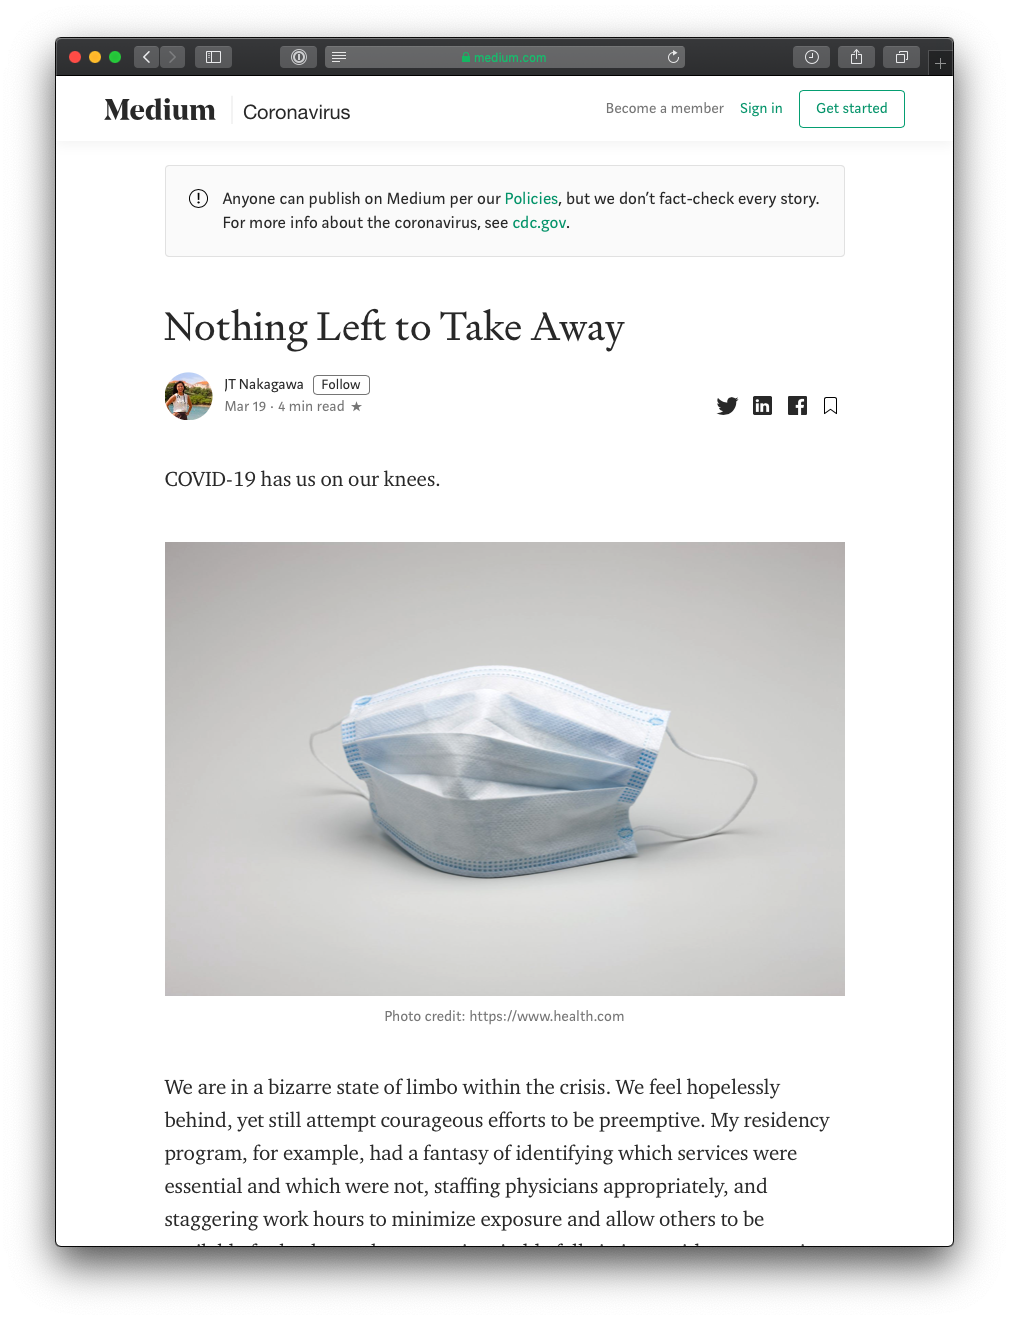
\includegraphics[width=.8\columnwidth]{voorbeeld-medium-desktop}
    \caption{Artikel op Medium weergegeven in een desktop-omgeving}
    \label{fig:ux-voorbeeld-medium:desktop}
\end{figure}

\begin{figure}
    \centering
    \subfloat[Donkere gebruikersomgeving]{{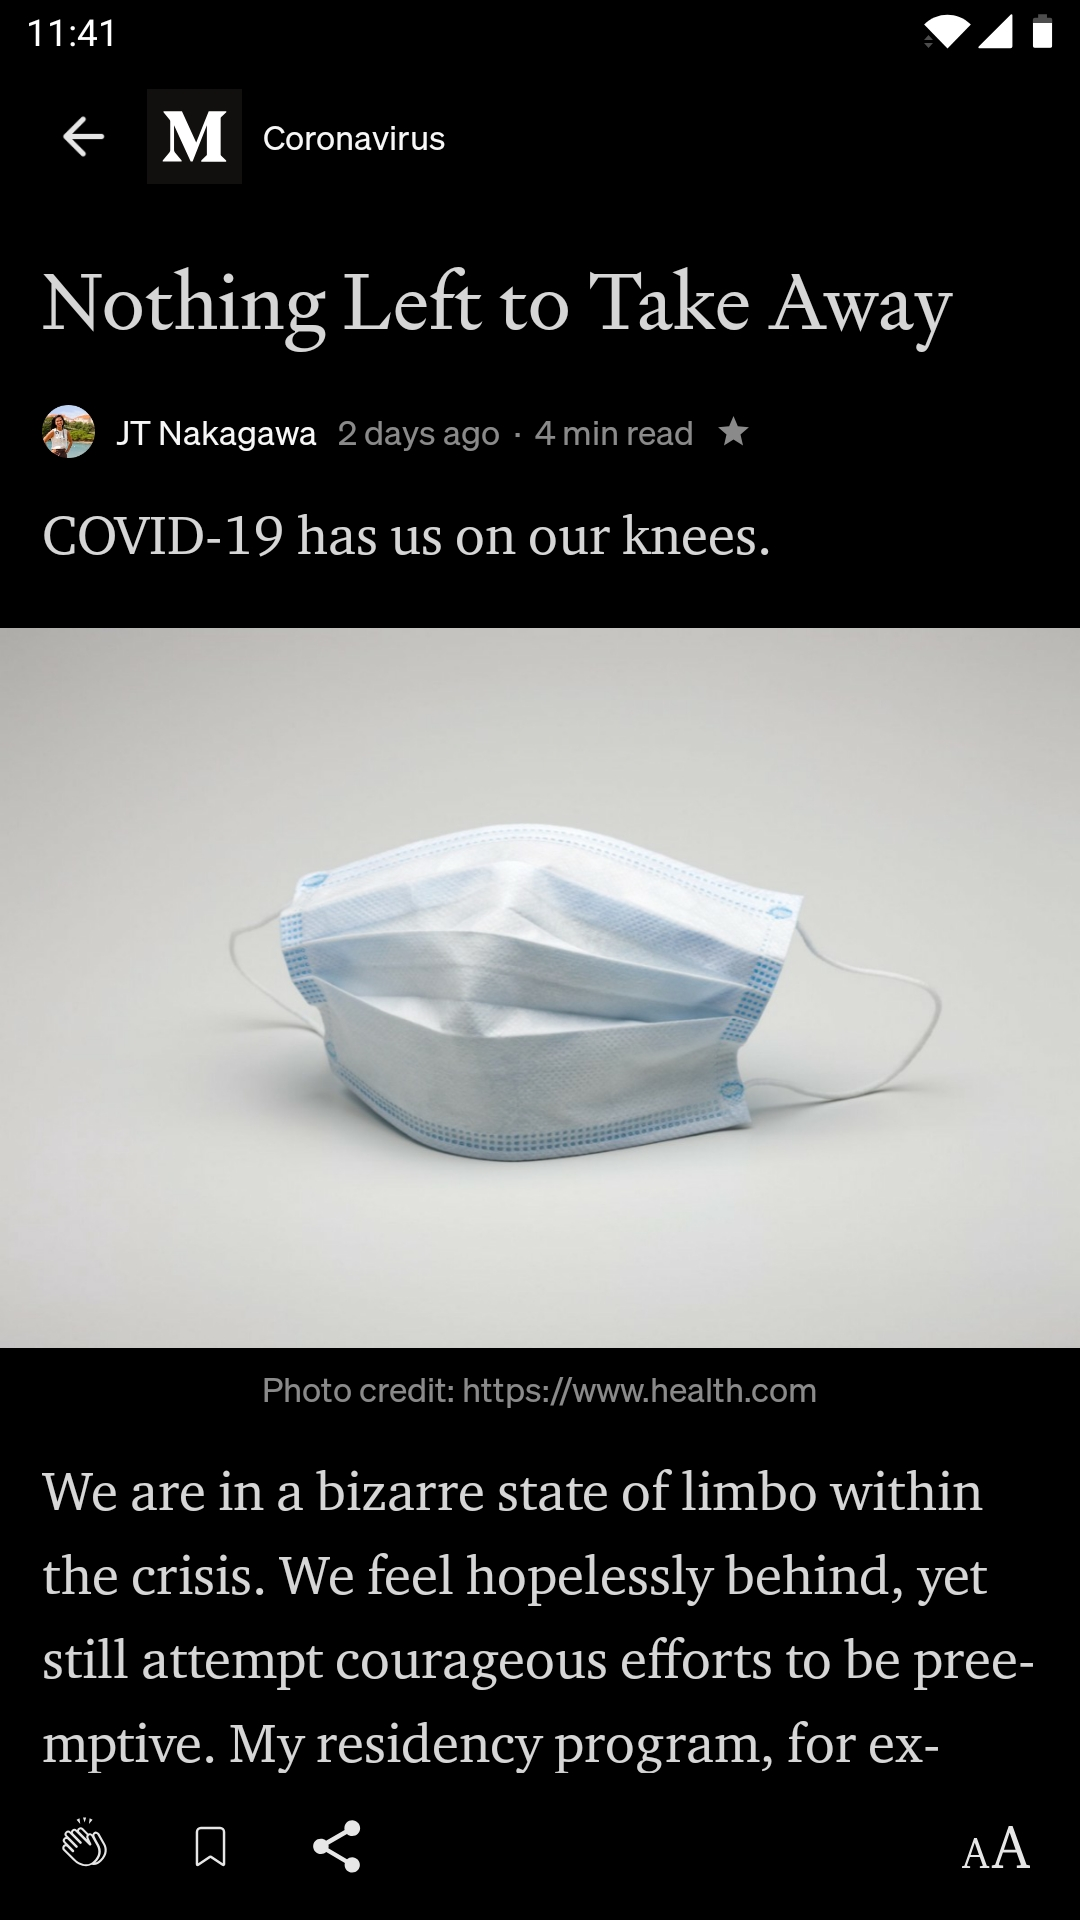
\includegraphics[width=.4\columnwidth]{voorbeeld-medium-mobiel-donker}}}
    \qquad
    \subfloat[Lichte gebruikersomgeving]{{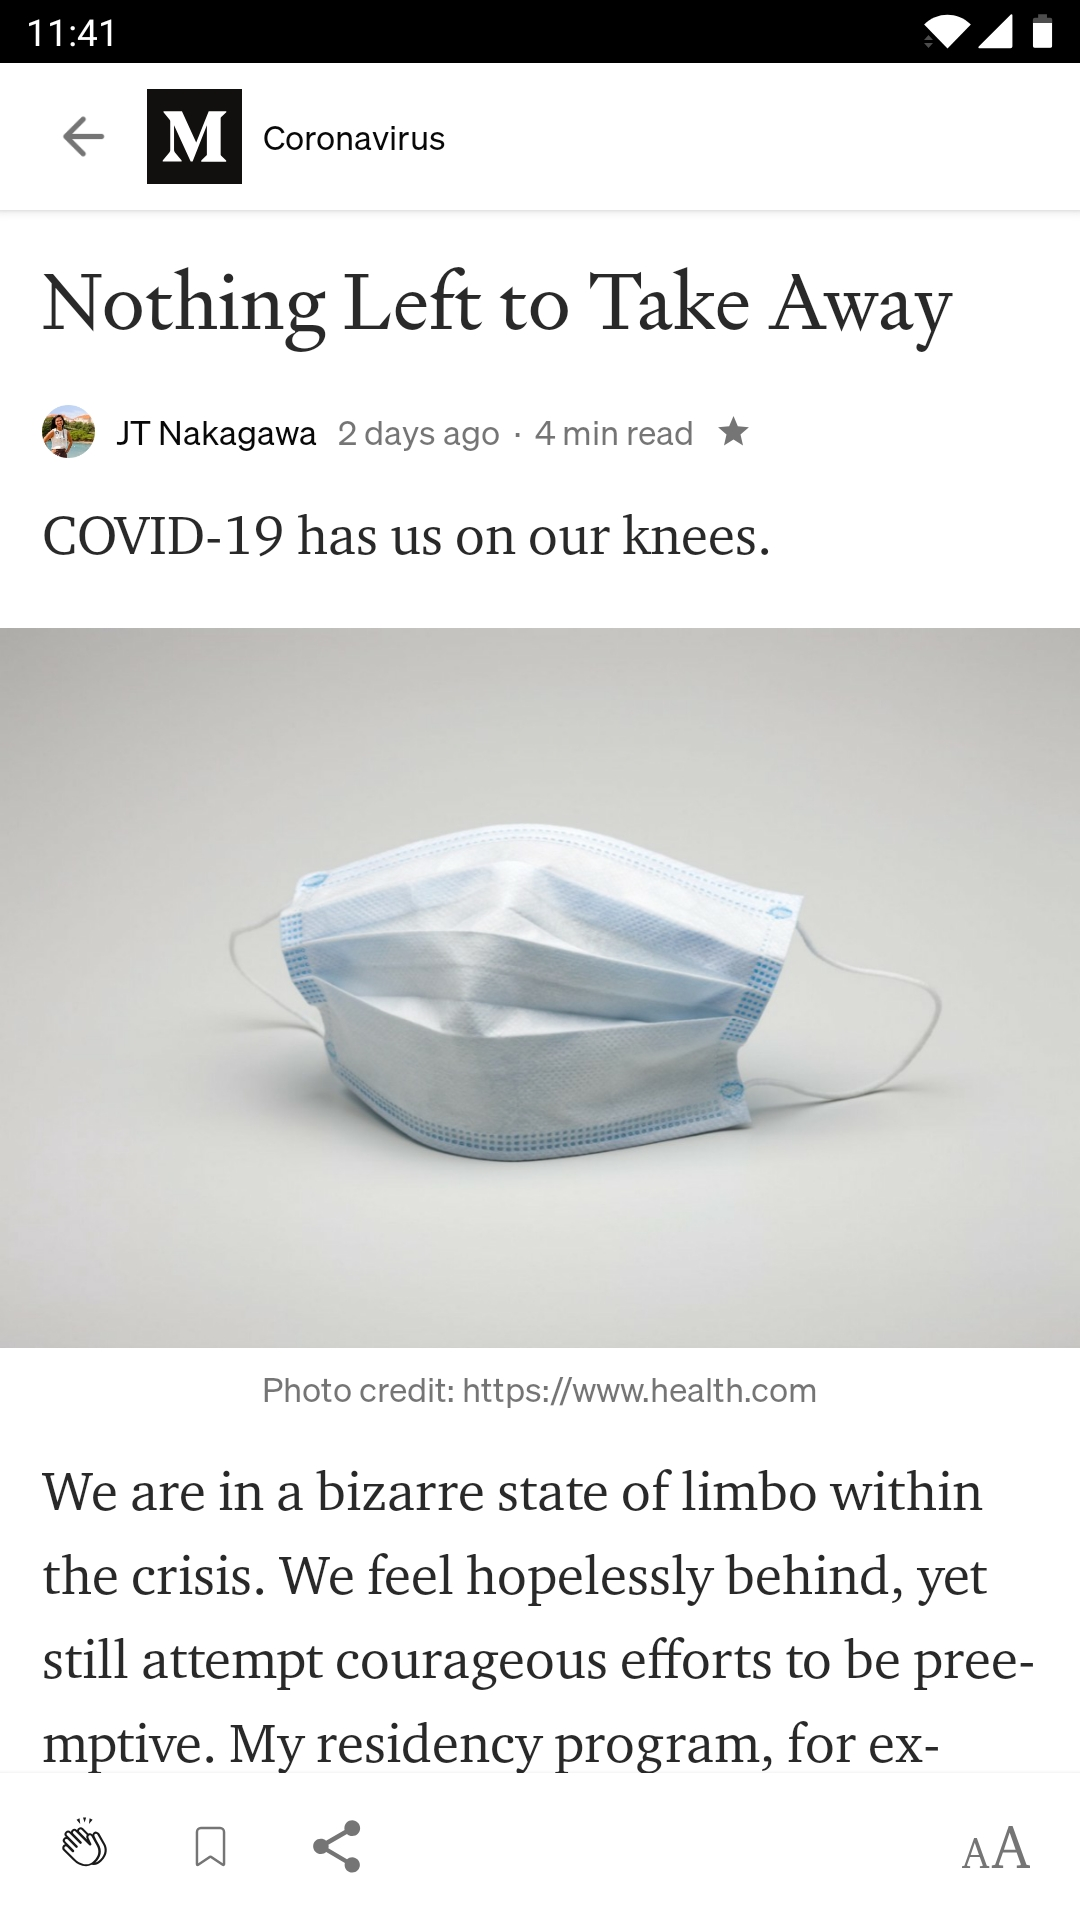
\includegraphics[width=.4\columnwidth]{voorbeeld-medium-mobiel-licht}}}
    \caption{Artikel op Medium weergegeven in een mobiele omgeving}
    \label{fig:ux-voorbeeld-medium:mobiel}
\end{figure}

\textbf{Airbnb} wil verkopen, dat is merkbaar van zodra je de website opent. Airbnb (\url{https://www.airbnb.com/}) is een platform waarmee je een kamer of woning van iemand anders kan huren voor een korte periode. Het is razend populair platform bij mensen die een plezier- of werkreis plannen en iets unieks zoeken of de kosten van hun reis willen drukken. Van zodra je op de homepagina komt zorgt Airbnb ervoor dat je onmiddellijk kan zoeken naar een geschikte plaats om te verblijven op een locatie en tijdstip naar keuze. Gepaard met een uitnodigende titel en een buitengewone afbeelding is de verleiding bij de gebruiker groot om hun ideale trip te beginnen plannen. Door deze directe aanpak vergeet de gebruiker als het ware de concurrentie van Airbnb, wat uiteraard net het doel was van bij het begin.

\begin{figure}
    \centering
    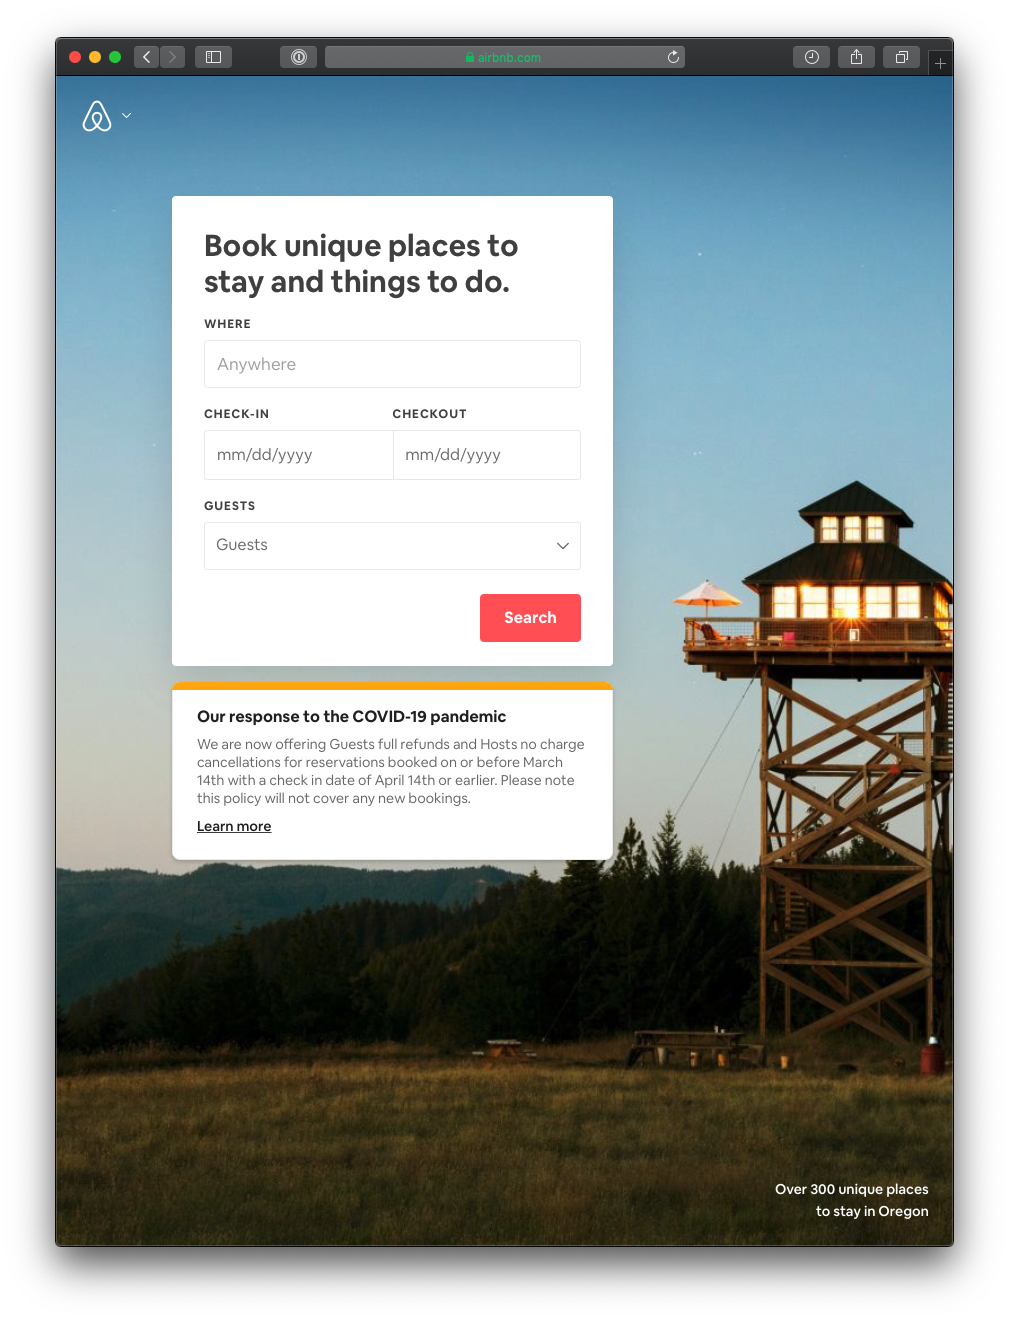
\includegraphics[width=.8\columnwidth]{voorbeeld-airbnb-desktop}
    \caption{Airbnb homepagina}
    \label{fig:ux-voorbeeld-airbnb}
\end{figure}

Slimme apparaten in het huishouden zijn bezig aan een opmars. Eén van de bekendste apparaten is de \textbf{Nest Smart Thermostat}, een slimme thermostaat die verbonden is met het internet. De thermostaat leert wanneer de ruimte moet opwarmen of afkoelen. Het fysieke toestel zelf is de simpliciteit zelve. Het is een grote, ronde knop met centraal de huidige temperatuur, indien de ruimtes opwarmen of afkoelen en de temperatuur waar men naartoe werkt. Een draai naar rechts en je verhoogt de gewenste temperatuur, een draai naar links en je verlaagt deze. De mobiele applicatie bootst deze werking na zodat de gebruiker zich direct comfortabel voelt met de interface (zie figuur~\ref{fig:ux-voorbeeld-nest}).

\begin{figure}
    \centering
    \subfloat[Fysiek toestel]{{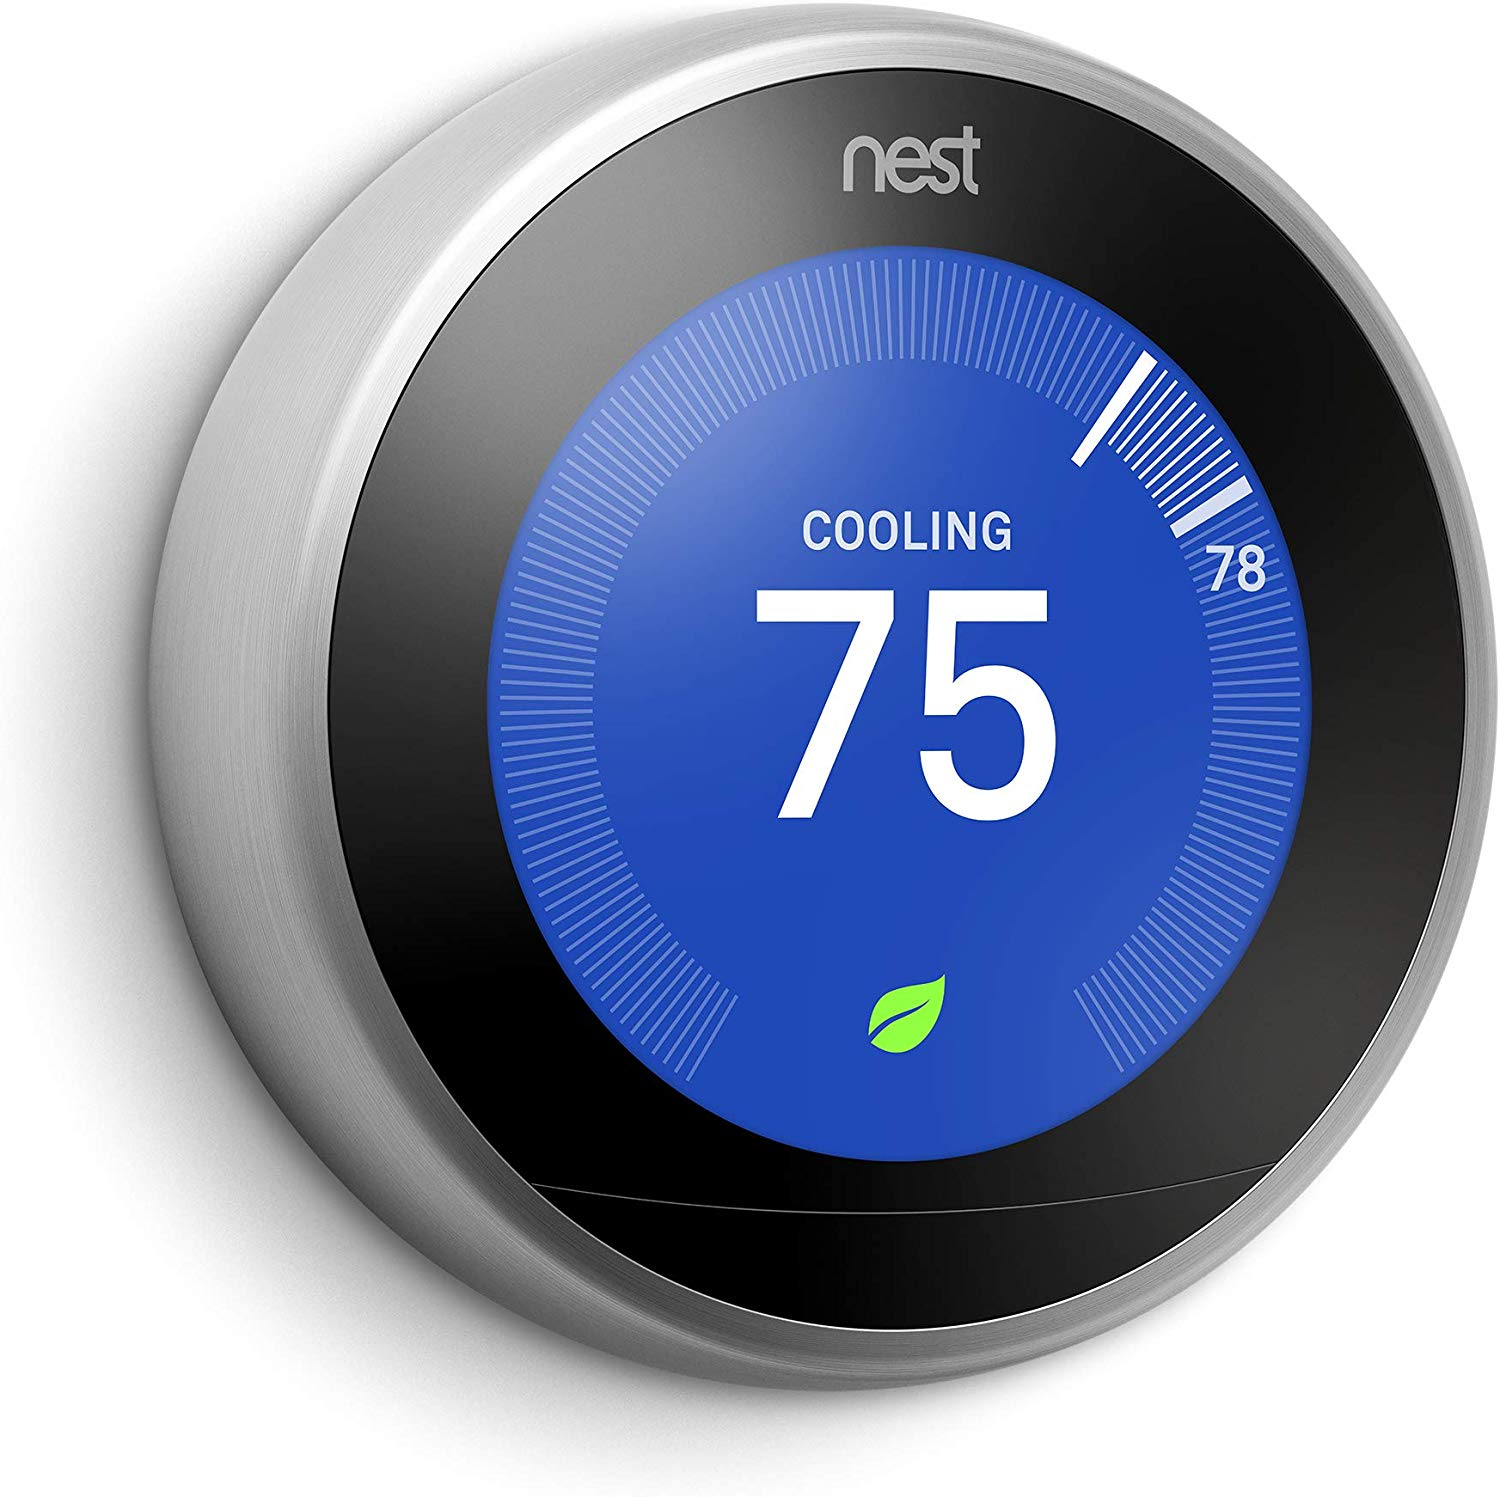
\includegraphics[width=.5\columnwidth]{voorbeeld-nest-toestel}}}
    \qquad
    \subfloat[Mobiele interface]{{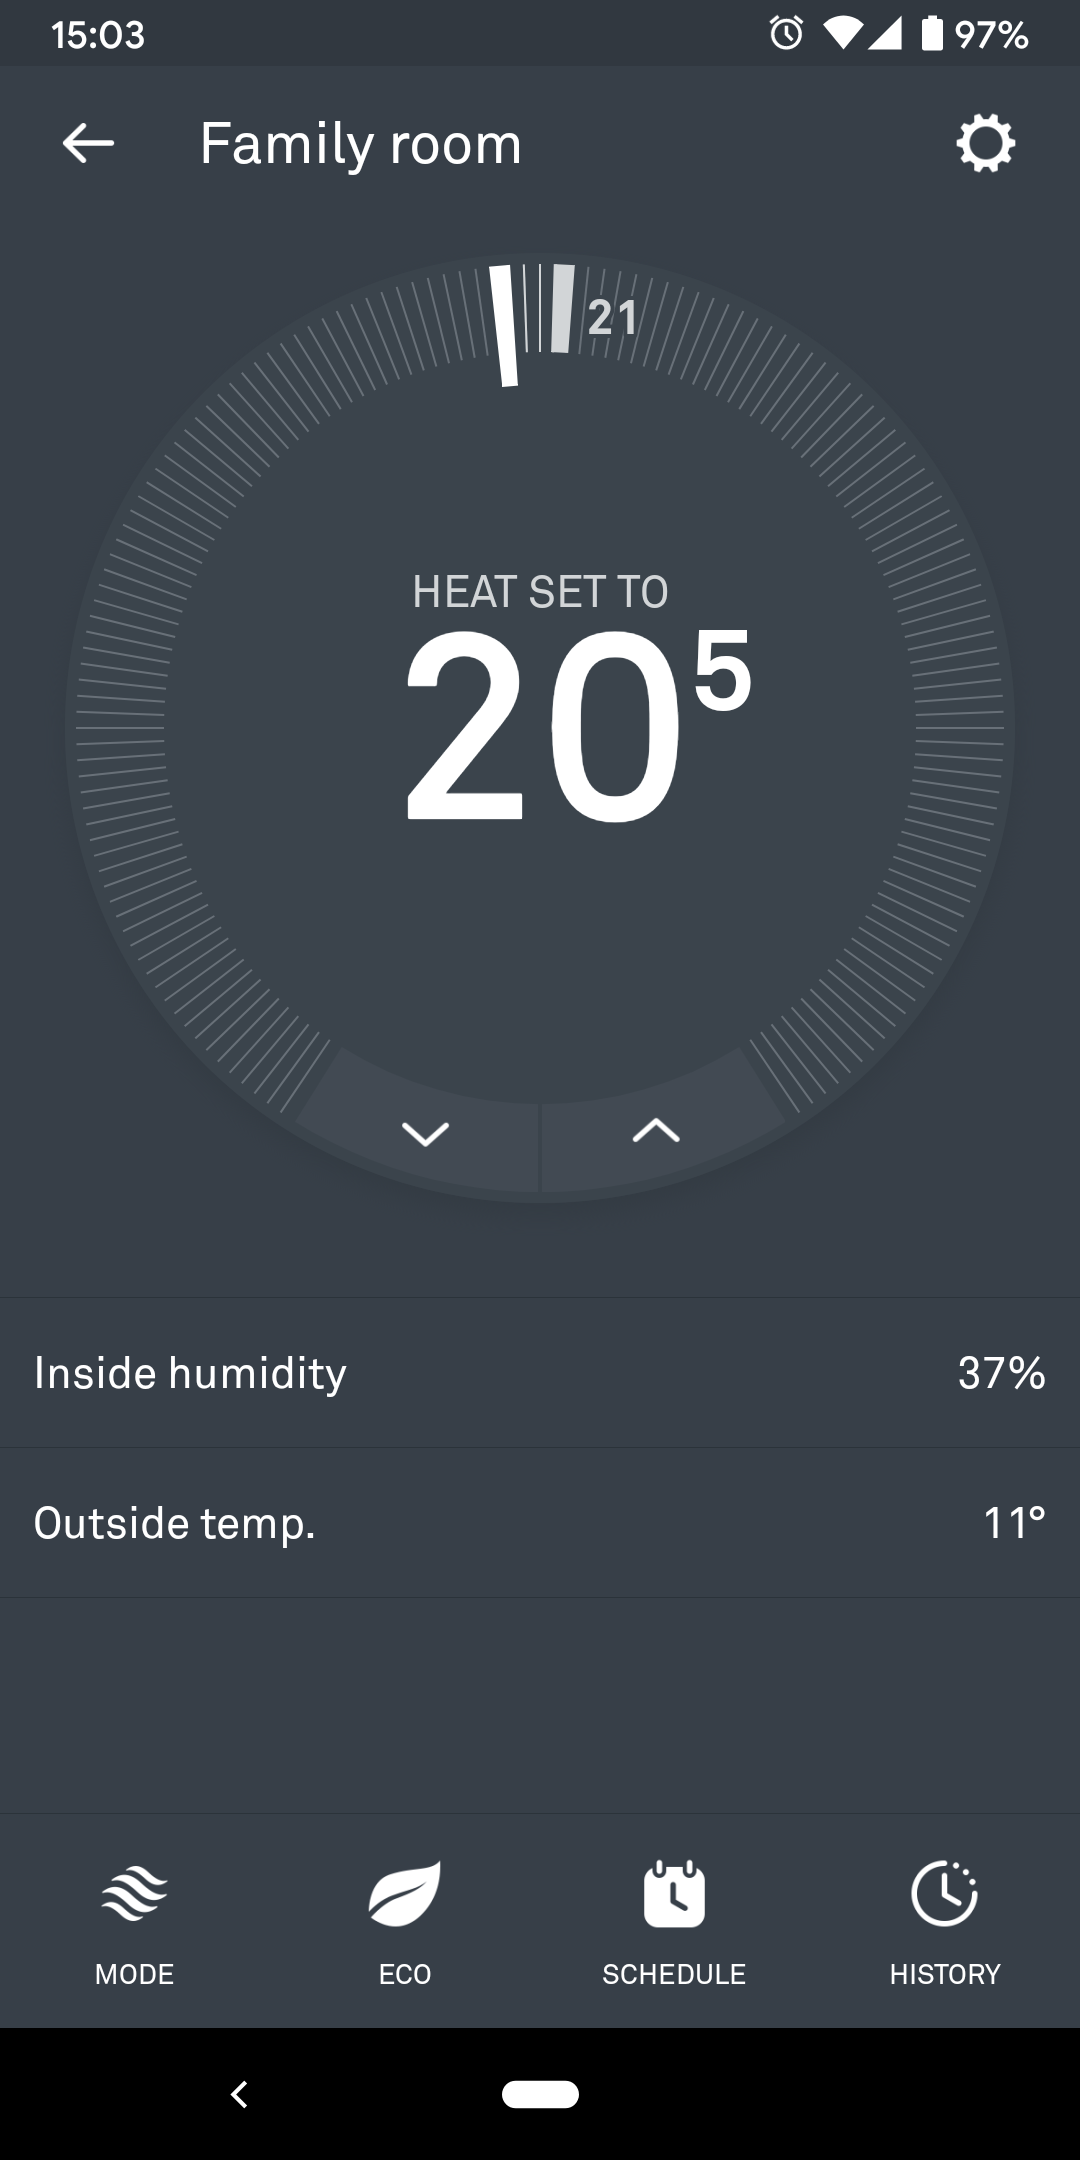
\includegraphics[width=.3\columnwidth]{voorbeeld-nest-mobiel}}}
    \caption{Nest Smart Thermostat}
    \label{fig:ux-voorbeeld-nest}
\end{figure}

\textbf{Hubspot} (\url{https://www.hubspot.com/}) maakt producten voor marketing, sales en klantenservice. Hubspot richt zich tot bedrijven van elke omvang. In dit voorbeeld bekijken we slechts een klein deel van de software. Binnen Hubspot is er de mogelijkheid om een massa-email te plannen die een deel van of alle klanten van de gebruiker bereikt. Uiteraard is dit een actie met een aanzienlijke impact op het bedrijf van de gebruiker. Een verzonden mail kan echter niet ongedaan gemaakt worden. Wanneer de gebruiker de email inplant komt Hubspot met een pop-up melding die toch nog even bevestiging vraagt (zie figuur~\ref{fig:ux-voorbeeld-hubspot}). Deze melding zorgt ervoor dat de kans op fouten verkleind wordt maar ook dat de gebruiker zich gerust voelt bij zijn acties.

\begin{figure}
    \centering
    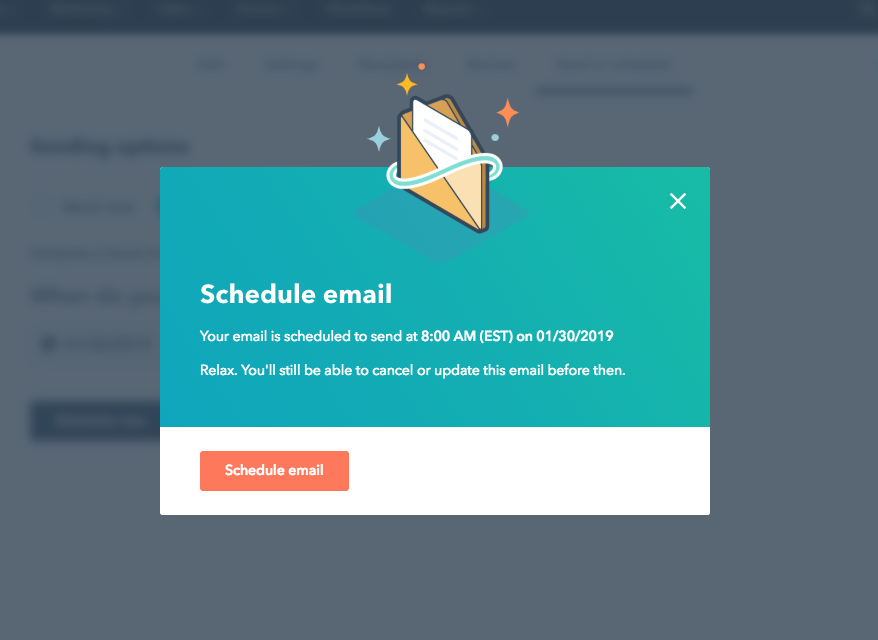
\includegraphics[width=.7\columnwidth]{voorbeeld-hubspot}
    \caption{Hubspot pop-up melding}
    \label{fig:ux-voorbeeld-hubspot}
\end{figure}

\section{Usability testing}
\label{sec:usability-testing}

Usability testing is een methode om alle onderdelen van de user experience honingraat (zie figuur~\ref{fig:ux-facets}) in een applicatie of website te testen. Men test de software in kwestie door er echte gebruikers op te laten werken en ondertussen hun handelingen te observeren. Het doel van usability testing is om de algemene gebruikerservaring te verbeteren~\autocite{Hotjar2020}.

Bij het creëren van software vergeet de ontwikkelaar al snel dat de gewone eindgebruiker vaak meer moeilijkheden zal ondervinden bij het gebruik van zijn creatie dan hijzelf. Doordat de ontwikkelaar hier zelf vaak blind voor is voert men testen uit met de eindgebruiker. Hierdoor kan men een beter inzicht krijgen over hoe bruikbaar de software is. In dit proces worden vaak vele euvels opgemerkt die anders in de productiesoftware zouden aanbelanden.
Zonder usability testing zou men vaak vast komen te zitten met een product dat het team van ontwikkelaars begrijpt, maar de doelgroep niet.

\subsection{Laboratory en field testing}
\label{sec:usability-testing:lab-field-testing}

In voorgaand onderzoek tonen \textcite{Kaikkonen2005} aan dat usability testing onderverdeeld kan worden in twee categorieën, namelijk laboratory en field testing. Laboratory testing houdt in dat men enkele testpersonen uitnodigt in testlabo's, dit is gewoonlijk op kantoor. Dit labo is een rustige ruimte waarin afleidingen beperkt zijn zodat de concentratie gegarandeerd kan worden. Ook al bestaan er veel twijfels rond laboratory testing, volgens \textcite{Kjeldskov2003} wordt het nog steeds vaker verkozen boven field testing. De reden achter deze keuze is vaak omdat men moeilijkheden ondervindt bij field testing. Het is eenvoudiger om testpersonen op te nemen en te observeren bij technieken zoals ``think aloud'' wanneer men gebruik maakt van laboratory testing.

Bij field testing worden te testpersonen uitgenodigd om de applicatie in kwestie te testen in de omgeving waar de applicatie normaal zou gebruikt worden. Een mobiele applicatie zoals \href{https://www.strava.com/}{Strava} die statistieken van lopers en fietsers bijhoudt zou bijvoorbeeld getest worden tijdens een trainingssessie. Sinds de opmars van de smartphone kan field testing steeds meer ingezet worden \autocite{Kjeldskov2004}. De camera die gebruikt wordt om de testsessie op te nemen wordt steeds kleiner, waardoor het field testing een pak aangenamer wordt.

In beide gevallen van usability testing werd geopteerd voor het ``think aloud'' protocol gebaseerd op het werk van \textcite{Ericsson1984}. Hierbij zal de testpersoon luidop denken. Dit zorgt ervoor dat er veel informatie vrijkomt over de gedachtegang van de gebruiker bij het gebruik van de applicatie. Dit kan makkelijk opgenomen worden om later conclusies uit te trekken.

\textcite{Kaikkonen2005} hebben ook kunnen afleiden dat zowel laboratory testing als field testing quasi dezelfde resultaten vertonen. In hun use case werden alle usability fouten bij beide testmethodes gevonden. Bij field testing vond men de fout som wel sneller of kwam men deze meerdere keren tegen.

\subsection{Andere testmethoden}
\label{sec:usability-testing:testmethoden}

Laboratory en field testing zijn slecht twee van vele methodes waarmee de bruikbaarheid van een applicatie kan getest worden. In een artikel van \textcite{Babich2019} worden de zeven belangrijkste methodes opgesomd.

% https://xd.adobe.com/ideas/process/user-testing/top-7-usability-testing-methods/

\subsubsection{Guerilla testing}
\label{sec:usability-testing:testmethoden:guerilla}

Guerilla testing is de eenvoudigste testmethode om zo snel mogelijk resultaten te krijgen. Bij guerilla testing gaat de moderator simpelweg op een publieke plaats aan willekeurige personen vragen om even het prototype van de applicatie te gebruiken. De moderator noteert dan de bevindingen. Guerilla testing voert men het best uit in het begin van het ontwikkelproces, zo weet men snel als men in de juiste richting werkt. Vaak krijgt de testpersoon een kleine attentie na het uitvoeren van de test. Zo kan de moderator bijvoorbeeld in een koffiebar plaatsnemen en testpersonen uitnodigen met een gratis koffie.

\subsubsection{Lab usability testing}
\label{sec:usability-testing:testmethoden:lab}

Deze testmethode werd eerder besproken in hoofdstuk~\ref{sec:usability-testing:lab-field-testing}. In contrast met geurilla testing kan men hier een gerichter publiek aantrekken en kan men zo relevantere informatie verkrijgen.

\subsubsection{Unmoderated remote usability testing}
\label{sec:usability-testing:testmethoden:unmoderated-remote}

Dit is een variant van field testing (zie hoofdstuk~\ref{sec:usability-testing:lab-field-testing}) zonder moderator. Hierbij gebruikt de testpersoon de applicatie in zijn omgeving en op zijn toestel. De informatie die men hierdoor verkrijgt is door het gebrek van een moderator natuurlijk beperkter. Het voordeel van deze methode is dat de kost lager is dan andere testmethoden.

\subsubsection{Contextual inquiry}
\label{sec:usability-testing:testmethoden:contextual-inquiry}

Deze methode leunt meer aan bij een observatiemethode dan bij een testmethode voor usability testing. De testpersonen krijgen hierbij een lijst met vragen die ze moeten beantwoorden over het product. Achteraf worden ze vaak gevraagd de applicatie te gebruiken in hun omgeving met een moderator (zoals bij field testing).

% TODO
